\documentclass[12pt]{article}
\usepackage[utf8]{inputenc}
\usepackage{graphicx} % Per includere immagini
\usepackage{titling}  % Per personalizzare lo spazio del titolo
\usepackage{ccicons}  % Per i simboli Creative Commons
\usepackage{geometry} % Per personalizzare i margini
\usepackage{hyperref} % Per i link
\usepackage[italian]{babel}
\usepackage{pgffor}
\usepackage{listings}
\usepackage{color}
\usepackage{float}
\usepackage{pdflscape}

\definecolor{codegreen}{rgb}{0,0.6,0}
\definecolor{codegray}{rgb}{0.5,0.5,0.5}
\definecolor{codepurple}{rgb}{0.58,0,0.82}
\definecolor{backcolour}{rgb}{0.95,0.95,0.92}

\lstdefinestyle{mystyle}{
    backgroundcolor=\color{backcolour},   
    commentstyle=\color{codegreen},
    keywordstyle=\color{magenta},
    numberstyle=\tiny\color{codegray},
    stringstyle=\color{codepurple},
    basicstyle=\ttfamily\footnotesize,
    breakatwhitespace=false,         
    breaklines=true,                 
    captionpos=b,                    
    keepspaces=true,                 
    numbers=left,                    
    numbersep=5pt,                  
    showspaces=false,                
    showstringspaces=false,
    showtabs=false,                  
    tabsize=2
}

\lstset{style=mystyle}

% Imposta i margini della pagina
\geometry{
  top=2cm,
  bottom=2cm,
  left=3cm,
  right=3cm
}

\lstset{
  basicstyle=\ttfamily,
  breaklines=true,
  columns=fullflexible
}

\setlength{\droptitle}{-5em} % Sposta in alto il titolo

\title{
    \Large \textbf{UNIVERSITA' DI SALERNO} \\[0.5em]
    \small DIPARTIMENTO DI INGEGNERIA DELL'INFORMAZIONE ED ELETTRICA E MATEMATICA APPLICATA\\[5em]
    
\includegraphics[width=0.6\textwidth]{logo_uni.png}\\[3em] % Logo dell'Università
    \normalsize Laurea Magistrale in Ingegneria Informatica \\[1em]
    \Large \textbf {Project work} \\[1em]
    \large \textbf {Deliverable 2} \\ [1em]
    \large {Sistemi Embedded} \\[1em]
}

\author{
    \textbf{Gruppo: 8} \\
    \normalsize Marotta Giuseppe - 0622702302 - g.marotta31@studenti.unisa.it\\
    \normalsize Rea Gaetano - 0622702190 - g.rea7@studenti.unisa.it\\
    \normalsize Squitieri Giuseppe - 0622702339 - g.squitieri8@studenti.unisa.it\\ 
    \normalsize Tramice Davide - 0622702194 - d.tramice@studenti.unisa.it\\ \\
    }

\date{
    ANNO ACCADEMICO 2023/2024 % Data
}

\begin{document}


\begin{titlingpage} % Crea una pagina di titolo personalizzata
\maketitle
\thispagestyle{empty} % Rimuove il numero di pagina
%\begin{center}
    %\ccbyncnd % Simbolo Creative Commons
%\end{center}
\end{titlingpage}

% Creazione di una nuova pagina
\newpage

% Aggiungi l'indice delle sezioni
\tableofcontents


\newpage

\section{Implementazione}

In accordo con la progettazione descritta nel capitolo precedente, in questo capitolo verrà dettagliata l'implementazione del modello Stateflow. Si inizierà con una panoramica generale, per poi scendere progressivamente a livelli di dettaglio sempre maggiori.

\subsection{Descrizione del Modello}

Il modello Stateflow è stato sviluppato per gestire i vari stati e le transizioni del sistema di controllo del cancello automatico. I principali componenti del modello includono:

\begin{itemize}
    \item \textbf{Sistema di Controllo del Cancello}: Gestisce gli stati di apertura, chiusura, controllo dei tempi e gestione degli ostacoli.
    \item \textbf{Pulsanti di Controllo}: Include i pulsanti B1, B2 e B3 per l'apertura/chiusura, la regolazione del tempo di chiusura e la regolazione del tempo di lavoro, rispettivamente.
    \item \textbf{Sensori di Ostacolo}: Sensori P1 e P2 per rilevare la presenza di ostacoli e per il controllo sulla chiusura completa del cancello.
    \item \textbf{Indicatori LED}: LED verde, giallo e rosso per indicare lo stato del cancello (aperto, chiuso, in movimento, errore).
\end{itemize}

\begin{figure}[H]
    \centering
    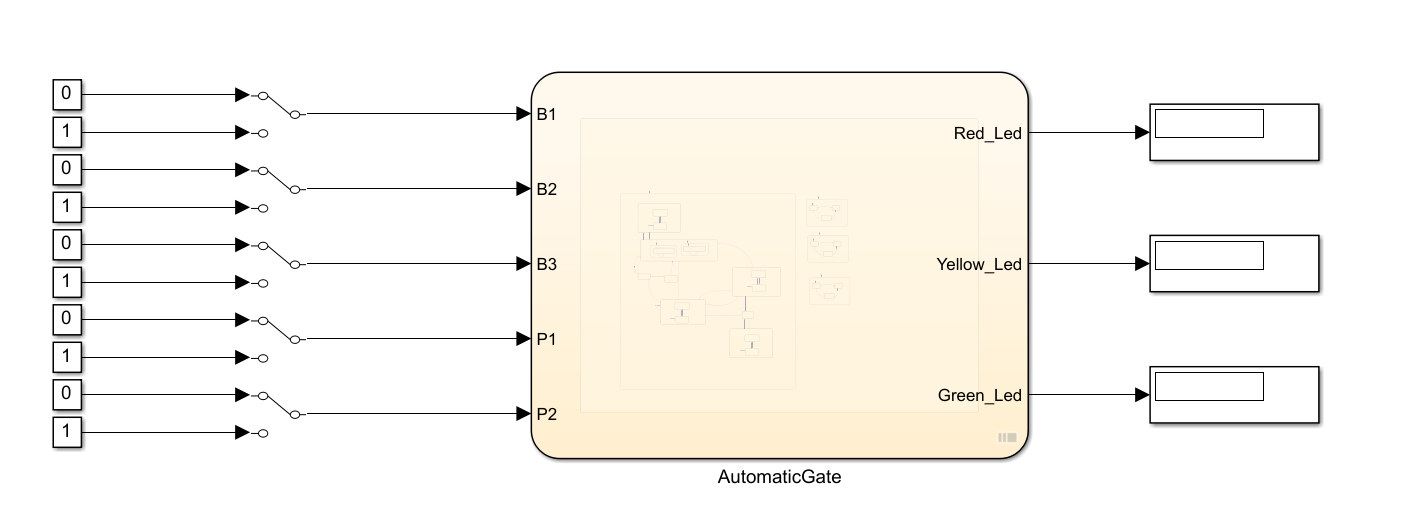
\includegraphics[width=1\textwidth]{imm/Vista_Generale.png}
    \caption{Vista Generale del Sistema.}
\end{figure}

\newpage

\noindent Di seguito vengono presentati gli input e gli output del sistema insieme alle costanti interne che vengono utilizzate per una corretta implementazione e un giusto funzionamento:

\begin{table}[H]
\centering
\begin{tabular}{|c|c|c|c|}
\hline
\textbf{Type} & \textbf{Name} & \textbf{Value} & \textbf{Port} \\ \hline
\texttt{Input\_Data} & B1 & - & 1 \\ \hline
\texttt{Input\_Data} & B2 & - & 2 \\ \hline
\texttt{Input\_Data} & B3 & - & 3 \\ \hline
\texttt{Output\_Data} & Red\_Led & - & 1 \\ \hline
\texttt{Output\_Data} & Green\_Led & - & 2 \\ \hline
\texttt{Output\_Data} & Yellow\_Led & - & 3 \\ \hline
\texttt{Input\_Data} & P1 & - & 4 \\ \hline
\texttt{Input\_Data} & P2 & - & 5 \\ \hline
\texttt{Constant\_Data} & BUTTON\_OFF & 0 & - \\ \hline
\texttt{Local\_Data} & WORK\_DUR & 10 & - \\ \hline
\texttt{Constant\_Data} & P\_ON & 1 & - \\ \hline
\texttt{Constant\_Data} & P\_OFF & 0 & - \\ \hline
\texttt{Local\_Data} & OPEN\_DUR & 10 & - \\ \hline
\texttt{Constant\_Data} & LED\_ON & 1 & - \\ \hline
\texttt{Constant\_Data} & LED\_OFF & 0 & - \\ \hline
\texttt{Constant\_Data} & BUTTON\_ON & 1 & - \\ \hline
\texttt{Constant\_Data} & EMER\_DUR & 10 & - \\ \hline
\texttt{Constant\_Data} & YELLOW\_DUR & 1 & - \\ \hline
\texttt{Constant\_Data} & GREEN\_DUR & 0.5 & - \\ \hline
\texttt{Constant\_Data} & EMER\_P1\_DUR & 30 & - \\ \hline
\texttt{Local\_Event} & B1\_PRESSED & - & - \\ \hline
\texttt{Local\_Event} & B2\_PRESSED & - & - \\ \hline
\texttt{Local\_Event} & B3\_PRESSED & - & - \\ \hline

\end{tabular}
\caption{Variabili utilizzate nel modello Stateflow}
\label{tab:variables}
\end{table}

\subsection{Introduzione al Core del Cancello}

Nel core del nostro sistema, troviamo vari stati che lavorano in parallelo: \textbf{Automatic Gate, B1, B2, B3}. Lo stato \textbf{Automatic Gate} gestisce tutta la logica di funzionamento del cancello, mentre gli altri stati gestiscono la corretta pressione dei rispettivi pulsanti.

\subsubsection{Pulsante B1}

Descriviamo nel dettaglio lo stato del pulsante B1. Questo componente viene utilizzato per richiedere l'apertura o la chiusura del cancello e sono previsti tre super-stati: \textbf{RELEASED, PRESSED, LONGPRESSED}.

\begin{enumerate}
    \item \textbf{RELEASED}: Stato iniziale. Si passa allo stato \textbf{PRESSED} quando viene rilevata la pressione del pulsante B1.
    \item \textbf{PRESSED}: Stato attivo durante la pressione del pulsante. Se viene rilevato un fronte di discesa, si passa allo stato \textbf{LONGPRESSED}.
    \item \textbf{LONGPRESSED}: Stato transitorio che, quasi istantaneamente, ritorna allo stato di \textbf{RELEASED}. Prima di tornare allo stato di \textbf{RELEASED}, viene eseguita un'azione che indica l'evento "B1\_pressed".
\end{enumerate}

\noindent Successivamente, descriveremo come questo evento impatta sulla logica di funzionamento nello stato \textbf{AUTOMATIC GATE}.

\begin{figure}[h]
    \centering
    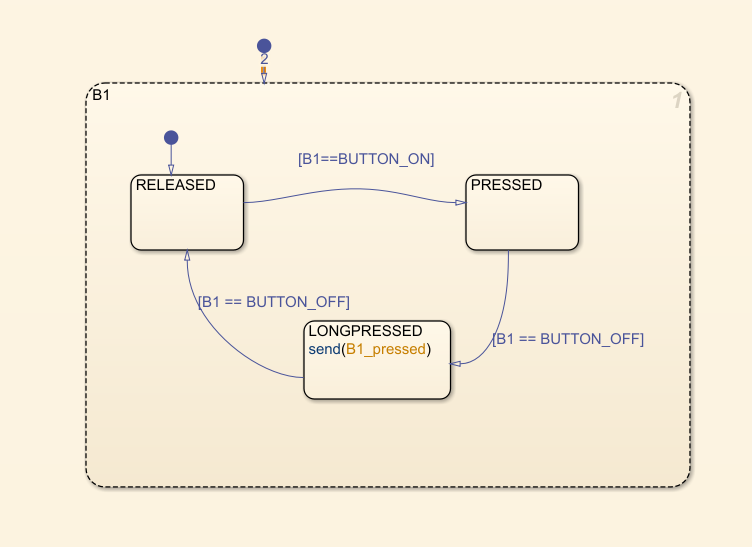
\includegraphics[width=0.7\textwidth]{imm/Pulsante_B1.png}
    \caption{Pulsante B1.}
\end{figure}
\newpage
\subsubsection{Pulsante B2 e B3}

Il Pulsante B2 è utile per regolare il tempo di chiusura automatica del cancello, mentre il pulsante B3 è usato per il settaggio dei valori del Tempo di Lavoro in fase di apertura e chiusura. Entrambi condividono lo stesso funzionamento del Pulsante B1 descritto precedentemente.

\begin{figure}[H]
    \centering
    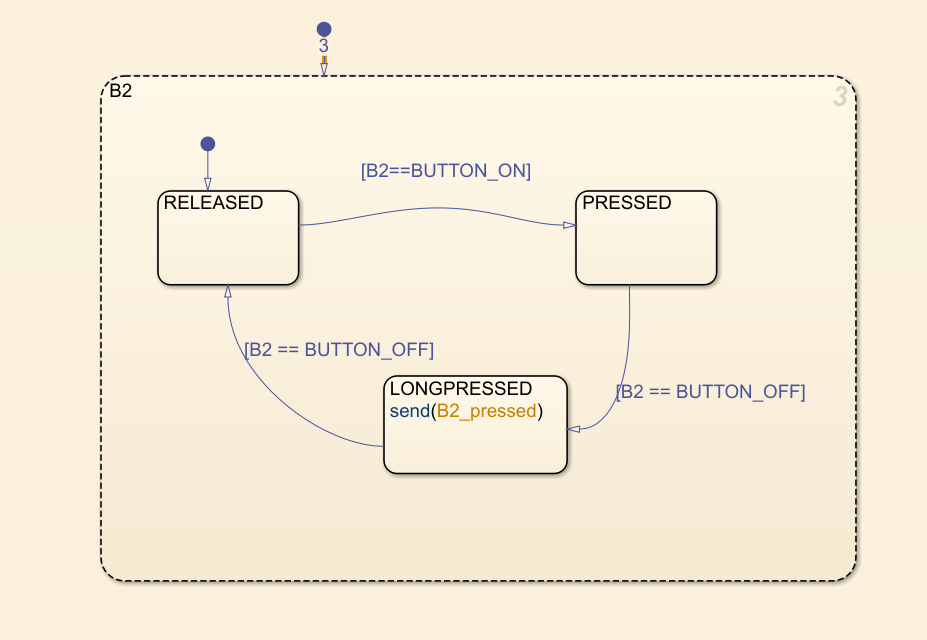
\includegraphics[width=0.8\textwidth]{imm/Pulsante_B2.png}
    \caption{Pulsante B2.}
\end{figure}

\begin{figure}[H]
    \centering
    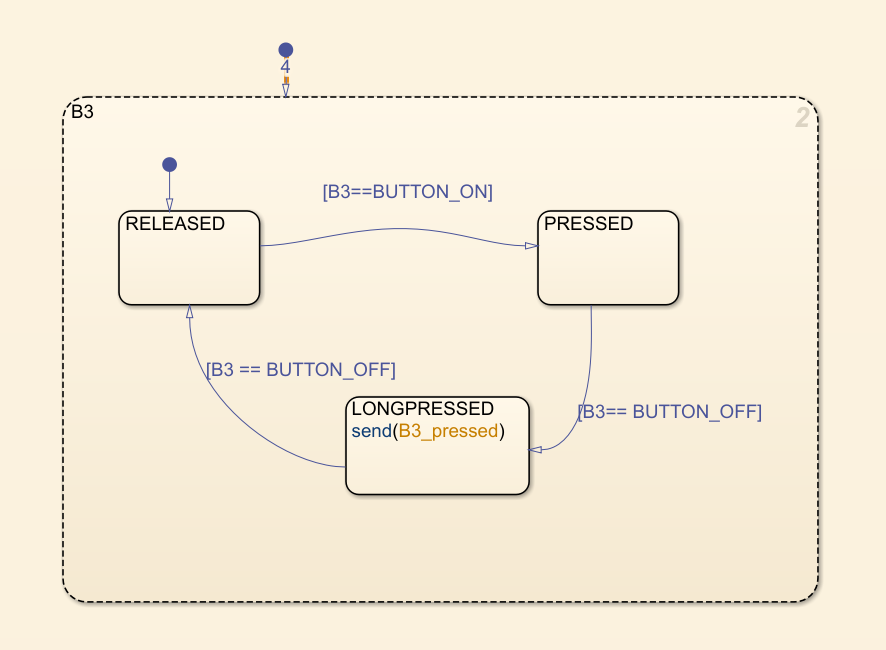
\includegraphics[width=0.8\textwidth]{imm/Pulsante_B3.png}
    \caption{Pulsante B3.}
\end{figure}

\subsubsection{Automatic Gate}

Arriviamo ora a descrivere lo stato che implementa la logica di funzionamento. Innanzitutto, come scelta implementativa, consideriamo come Stato Iniziale lo stato \textbf{CLOSING}. Consideriamo quest'ultimo tale poiché le specifiche richiedono che al momento dell'attivazione del sistema, se il cancello è aperto, ovvero P2 è inattivo, quest'ultimo passi in uno stato di chiusura descritto appunto dal suddetto stato. All'interno troviamo due super-stati \textbf{YELLOW\_ON} e \textbf{YELLOW\_OFF} che descrivono il Toggle del LED Giallo che avviene con frequenza 0.5 Hz.

\begin{figure}[H]
    \centering
    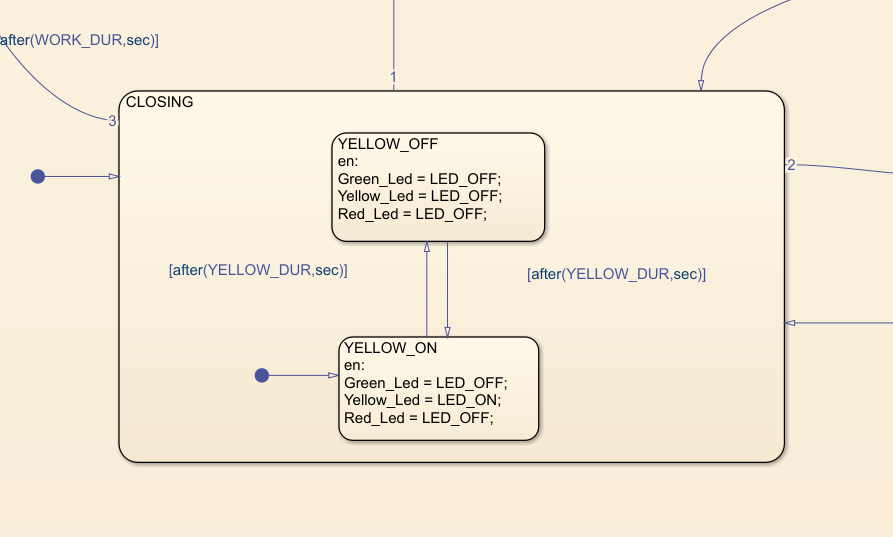
\includegraphics[width=0.6\textwidth]{imm/Closing.png}
    \caption{Closing State.}
\end{figure}

\noindent Nel momento in cui il cancello si chiude completamente o è già chiuso (P2 è attivo), si passa allo stato \textbf{CLOSED}. In questo stato, tutti i LED sono spenti e al suo interno troviamo due super-stati: \textbf{OPEN\_DUR\_SETTING} e \textbf{WORK\_DUR\_SETTING} che descrivono il settaggio dei parametri del tempo di chiusura automatica e del tempo di lavoro, che può essere attuato solo se il sistema si trova in questo stato. Per descrivere questi stati interni prenderemo in esame \textbf{OPEN\_DUR\_SETTING}, poiché il discorso è analogo per \textbf{WORK\_DUR\_SETTING}. Quando viene premuto B2, viene generato un evento che poi viene catturato da quest'ultimo stato e viene effettuata un'operazione che modifica la variabile \textbf{OPEN\_DUR}: 

\[
\mathrm{OPEN\_DUR} = \mathrm{mod}((\mathrm{OPEN\_DUR}), 120) + 10
\]

Questo perché i valori impostati hanno un range (10, 120).

\begin{figure}[H]
    \centering
    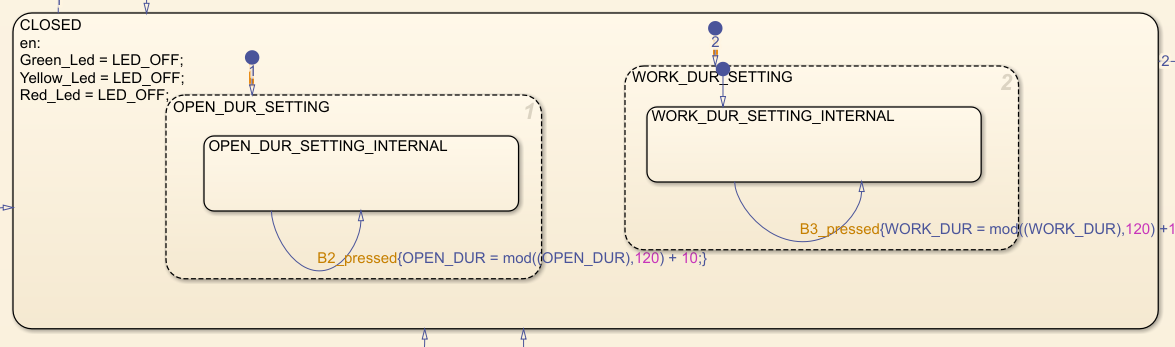
\includegraphics[width=0.8\textwidth]{imm/Closed.png}
    \caption{Closed State.}
\end{figure}

\noindent Chiaramente dallo stato di \textbf{CLOSED} si passa a \textbf{OPENING} nel momento in cui viene premuto B1. Al suo interno troviamo il Toggling del LED Giallo con lo stesso meccanismo di \textbf{CLOSING}.

\begin{figure}[H]
    \centering
    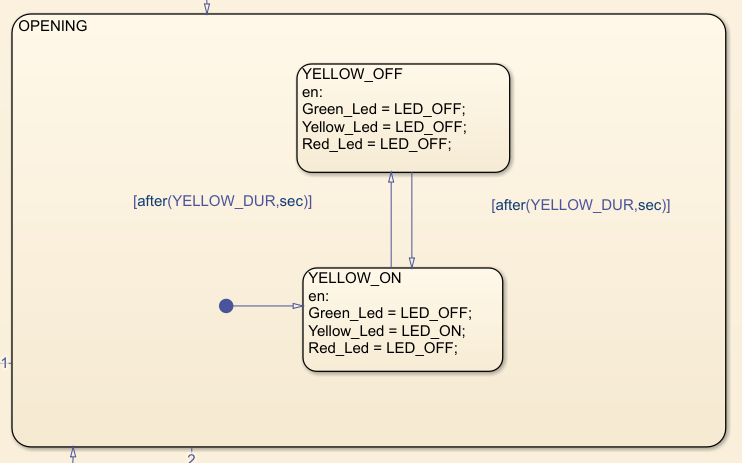
\includegraphics[width=0.5\textwidth]{imm/Opening.png}
    \caption{Opening State.}
\end{figure}

\noindent Appena finito il tempo di lavoro, il cancello va nello stato \textbf{OPEN} dove tutti i LED sono accesi.

\begin{figure}[H]
    \centering
    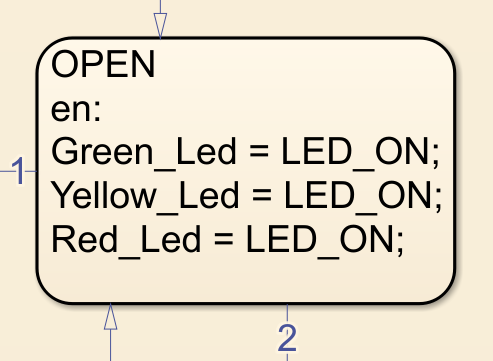
\includegraphics[width=0.3\textwidth]{imm/Open.png}
    \caption{Open State.}
\end{figure}
\newpage

\subsubsection{Emergency States}

Dallo stato \textbf{OPEN}, per tornare di nuovo in uno stato di chiusura, è possibile premere il pulsante B1 o attendere la chiusura automatica. Tuttavia, come specificato, il cancello non eseguirà il comando di chiusura se il sensore P1 è attivo, ma passerà nello stato \textbf{EMERGENCY\_P1\_OPEN}. Il sistema rimane in questo stato per 30 secondi o finché il sensore P1 non ritorna inattivo. Al suo interno troviamo due super-stati che descrivono il toggling del LED verde: \textbf{GREEN\_ON} e \textbf{GREEN\_OFF} con frequenza 1 Hz.
\vspace{1.5cm}
\begin{figure}[H]
    \centering
    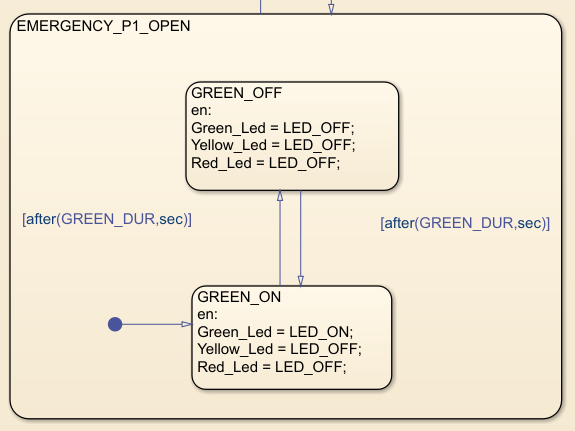
\includegraphics[width=0.5\textwidth]{imm/Emergency_P1_Open.png}
    \caption{Emergency P1 Open State.}
\end{figure}
\vspace{1.5cm}
\noindent Se P1 è attivo quando il cancello è chiuso e viene premuto il pulsante B1, il sistema passerà in uno stato analogo: \textbf{EMERGENCY\_P1\_CLOSED}.
\vspace{1cm}
\begin{figure}[H]
    \centering
    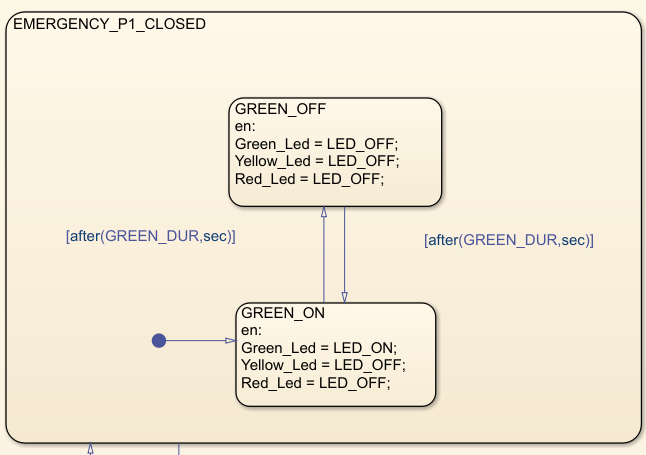
\includegraphics[width=0.5\textwidth]{imm/Emergency_P1_Closed.png}
    \caption{Emergency P1 Closed State.}
\end{figure}

\noindent Infine, descriviamo due stati che indicano una situazione di emergenza più grave (vero e proprio malfunzionamento del sistema): \textbf{EMERGENCY} e \textbf{EMERGENCY\_LED}. Lo stato \textbf{CLOSING} può durare al massimo un tempo T di lavoro, oltrepassato il quale, se P2 non è attivo, il sistema va in un primo stato \textbf{EMERGENCY} dove tutti i LED sono spenti e rimane per 10 secondi. Trascorsi questi 10 secondi, se P2 non è attivo, il sistema passa nello stato \textbf{EMERGENCY\_LED} dove è attivo il LED di emergenza rosso.

\begin{figure}[H]
    \centering
    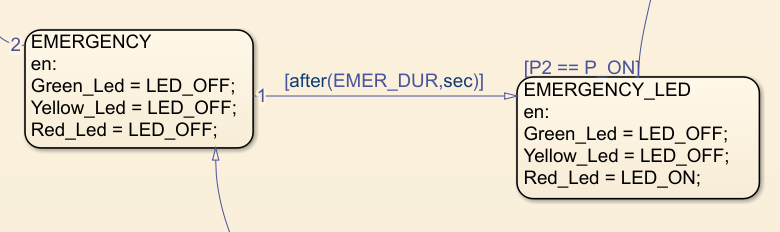
\includegraphics[width=1\textwidth]{imm/Emergency.png}
    \caption{Emergency State.}
\end{figure}

\newpage
\section{Testing}

In questo capitolo verranno illustrate le modalita per effettuare il testing del sistema. Questa parte è fondamentale per assicurarsi che non ci siano errori concettuali all'interno del modello e consegnare alla fase implementativa un progetto completo e senza imprecisioni.\\
Per testare lo State Model in Simulink si è utilizzato il tool Simulink Test che permette di descrivere procedure di testing in maniera agevole e soprattutto riproducibili. \\
Di seguito verranno descritti tutti i casi di test eseguiti che coprono quasi totalmente il sistema.

\subsection{Note al Testing}
Dopo un'attenta revisione, ci siamo resi conto che gli Activity diagrams attuali includono un numero eccessivo di casi differenti. Questo approccio, seppur inizialmente pensato per essere completo, ha reso la fase di test su Simulink Test estremamente complessa e difficile da gestire.\\
Per rendere i test più efficaci e praticabili, abbiamo deciso di spezzare i diagrammi di attività in parti più piccole e specifiche. Questo permetterà di isolare e testare singolarmente i vari casi, facilitando l'identificazione di eventuali problemi e migliorando la qualità complessiva del progetto.\\
Riteniamo che questa suddivisione ci consentirà di ottenere una validazione più accurata del sistema, garantendo al contempo una gestione più agevole dei test su Simulink Test.

\subsection{Test Case1: Opening/Closing}
In questo primo scenario testiamo il corretto funzionamento del sistema, dalla fase di chiusura fino a quando è chiuso e poi dalla fase di apertura fino a che non è completamente aperto. Questo test e molti dei successivi possono essere eseguiti molteplici volte ciclicamente.

\begin{itemize}
    \item Il cancello automatico parte da uno stato di chiusura in cui la fotocellula \textbf{P2} non rileva nulla. In questa fase viene testato il blinking del led giallo (yellow\_led).
    \item La fotocellula viene occupata entro il tempo di lavoro e quindi il cancello passa nello stato \textbf{CLOSED}. In questo stato si controlla che tutti i led siano spenti.
    \item Viene richiesta l'apertura del cancello generando un fronte di salita e poi uno di discesa con il segnale del pulsante \textbf{B1}
    \item Il cancello passa nello stato di \textbf{OPENING} durante il quale viene di nuovo testato se il blinking avviene alla frequenza giusta.
    \item Quando è passato il tempo di lavoro, inizialmente impostato a 10 secondi, si controlla che tutti i led siano accesi e che quindi il sistema si trova nello stato \textbf{OPEN}.
    \item Quando il sistema è nello stato open si avvia un timer che quando è scaduto fa passare il sistema nello stato \textbf{CLOSING}
    \item A questo punto si può ripartire dal primo punto e ripetere il test.
\end{itemize}

Di seguito in Figura 12 è presente il test in Simulink Test.

\begin{figure}[H]
    
    \hspace{-2.3cm} % Sposta l'immagine di 2 cm a sinistra
    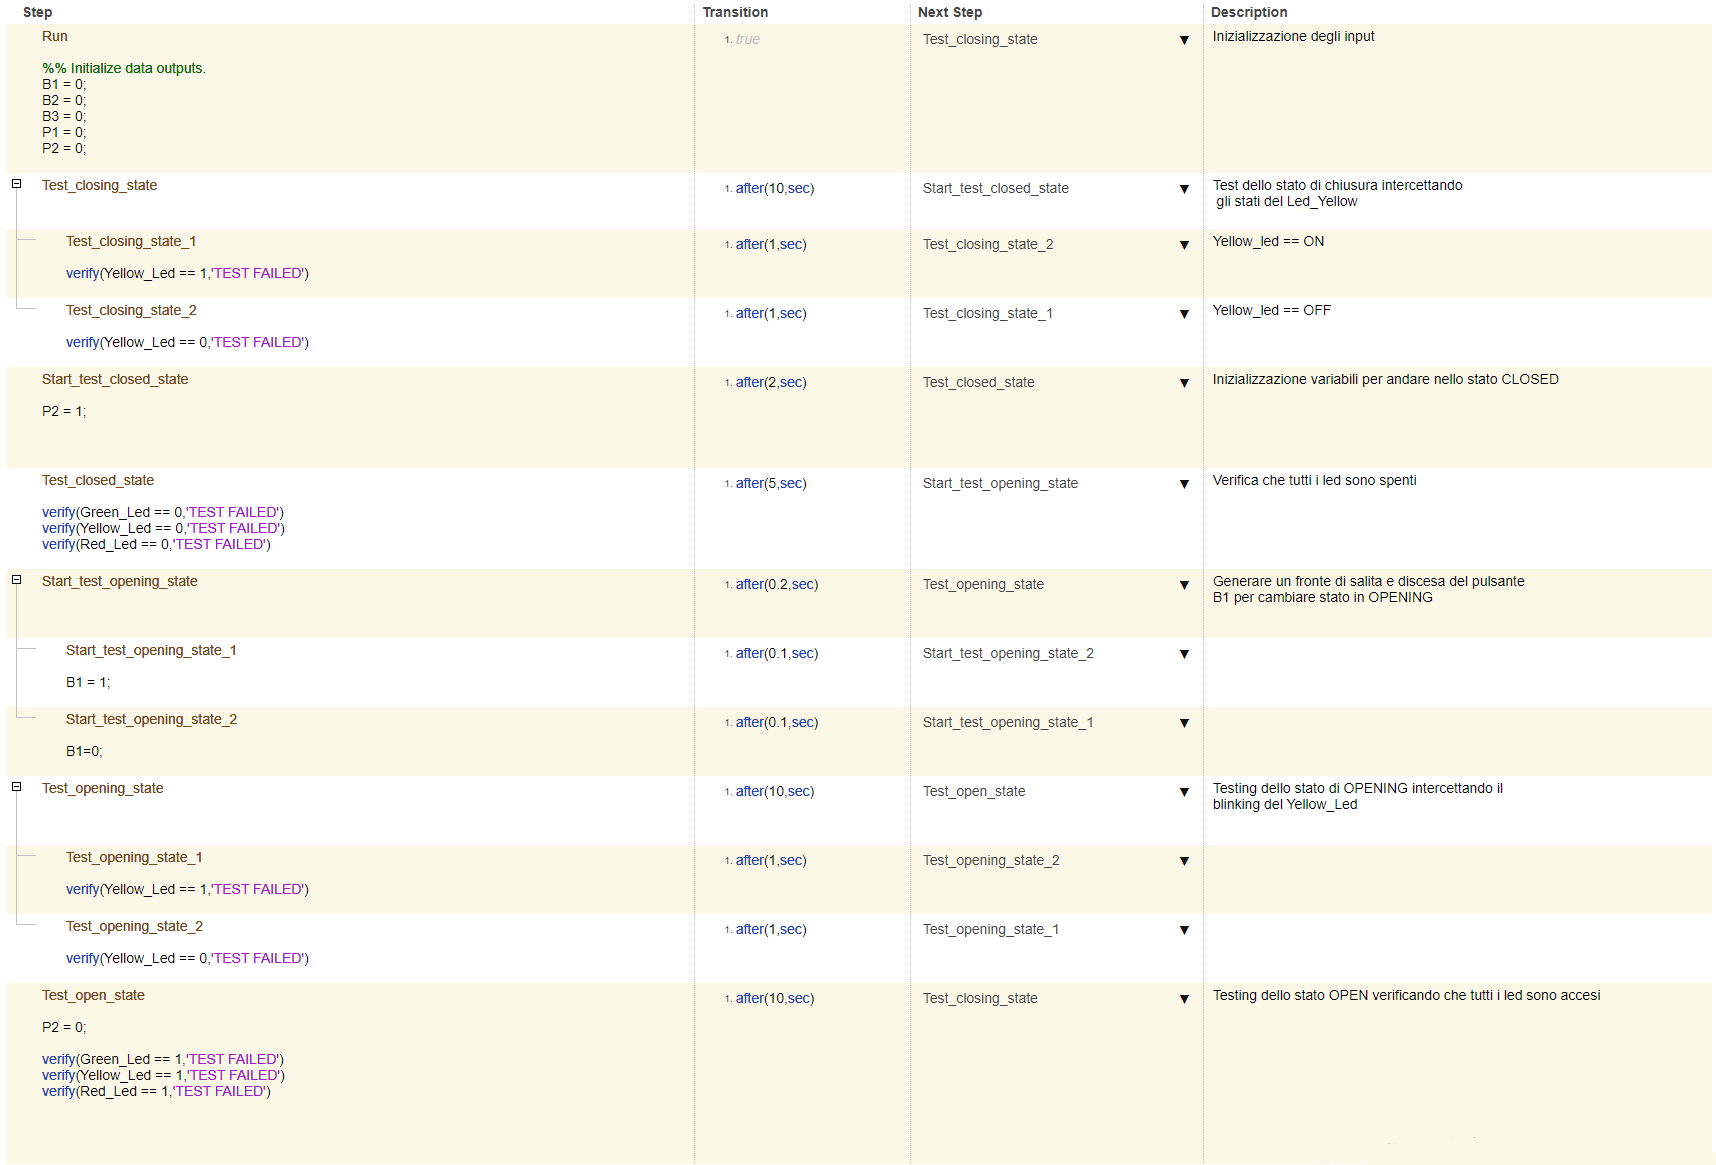
\includegraphics[width=1.3\textwidth]{Immagini_Test/Test_1_img.PNG}
    \caption{Test 1.}
    \label{fig:Test_1}
\end{figure}
\newpage
\subsection{Test Case 2: Opening emergency (P1 is ON)}

Il secondo scenario testa l'entrata e le uscite da uno degli stati di emergenza del cancello automatico, in particolare quello nel quale entra dallo stato \textbf{CLOSED} quando viene richiesta l'apertura, ma il sensore \textbf{P1} è impegnato.

\begin{itemize}
    \item Il sistema parte dallo stato \textbf{CLOSING}, quindi per eseguire il test viene portato nello stato \textbf{CLOSE} attivando \textbf{P2}.
    \item Viene controllato l'output del sistema in modo tale da assicurarsi che il cancello sia veramente chiuso.
    \item Si attiva la fotocellula con il valore 1 e successivamente, come nel caso precedente, si richiede l'apertura tramite \textbf{B1}. Il risultato atteso è quello che il led verde (Green\_Led) lampeggi ad una frequenza di 1Hz per 30 secondi se P1 rimane attiva o che si ritorni nello stato \textbf{CLOSED} appena c'è un fronte di discesa.
    \item Il primo caso di uscita testato è quello che utilizza il timer impostato a 30 sec.
    \item Per testare la seconda uscita si forza il sistema a rientrare nello stato di emergenza e poi si disattiva \textbf{P1}.
    \item Entrambi i test sono stati superati dal sistema.
\end{itemize}

In Figura 13 è rappresentato il test nella sua interezza. Si noti come sarebbe stato dispendioso utilizzare due casi di test separati per un solo stato di emergenza raggiungibile.

\begin{figure}[H]
    
    \hspace{-2.3cm} % Sposta l'immagine di 2 cm a sinistra
    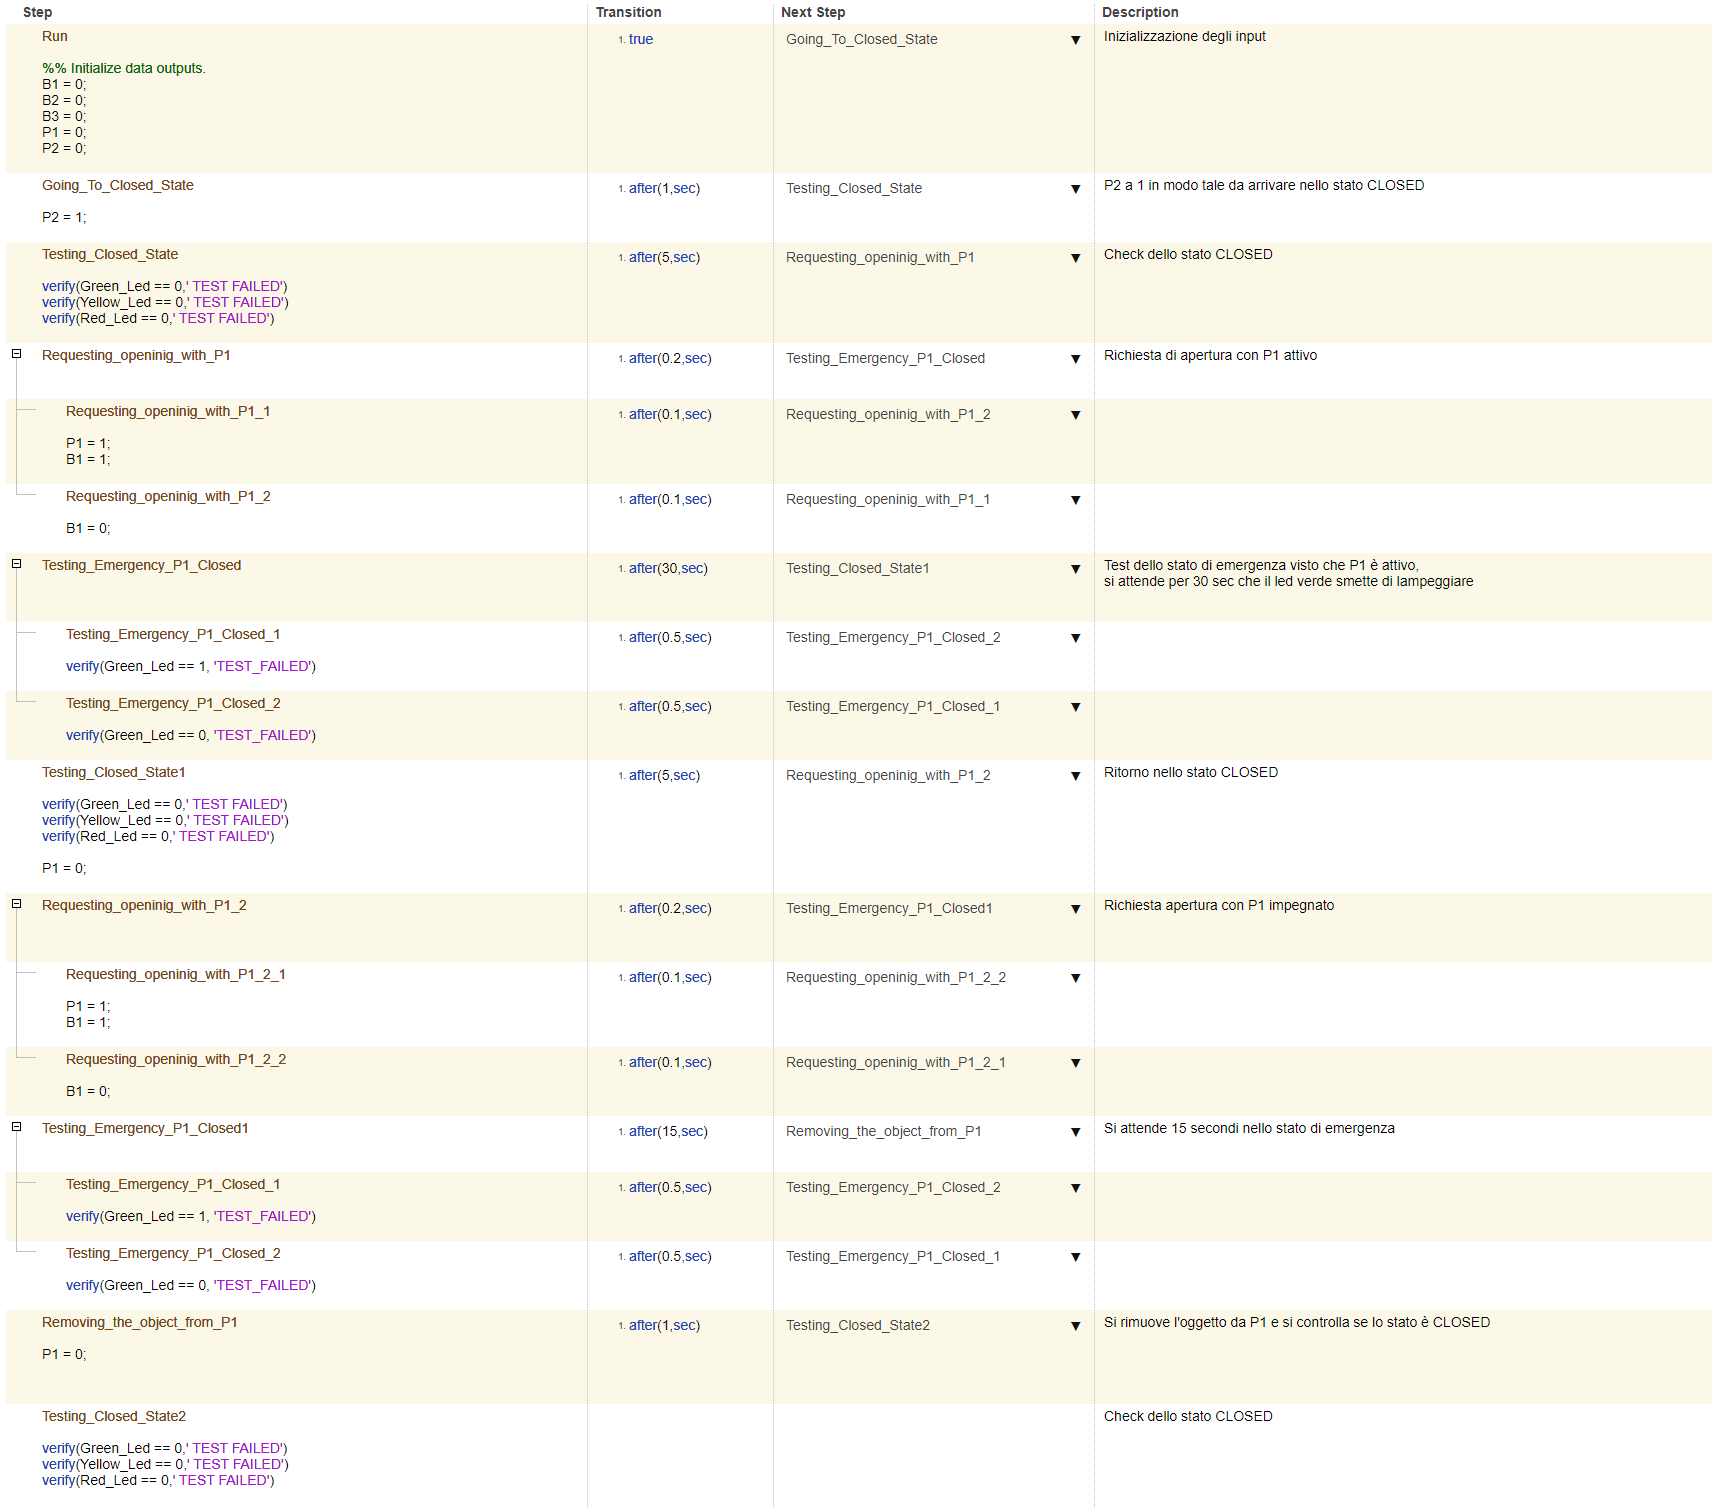
\includegraphics[width=1.3\textwidth]{Immagini_Test/Test_2_img.PNG}
    \caption{Test 2.}
    \label{fig:Test_2}
\end{figure}

\subsection{Test Case 3: Closing emergency (P1 is ON)}

Questo caso di test rappresenta una condizione di emergenza simile alla precedente, ma raggiungibile solo dallo stato \textbf{OPEN}. La descrizione è del tutto simile a quella sopra quindi si è scelto di ometterla. \\
Di seguito è riportato il caso di test in Figura ... .\\
Si sottolinea inoltre che la frequenza di lampeggio e le condizioni di uscita dallo stato di emergenza sono identiche al caso precedente.

\begin{figure}[!htbp]
    \vspace{-1cm} % sposta l'immagine di 1 centimetro verso l'alto
    \hspace{-2.3cm} % Sposta l'immagine di 2 cm a sinistra
    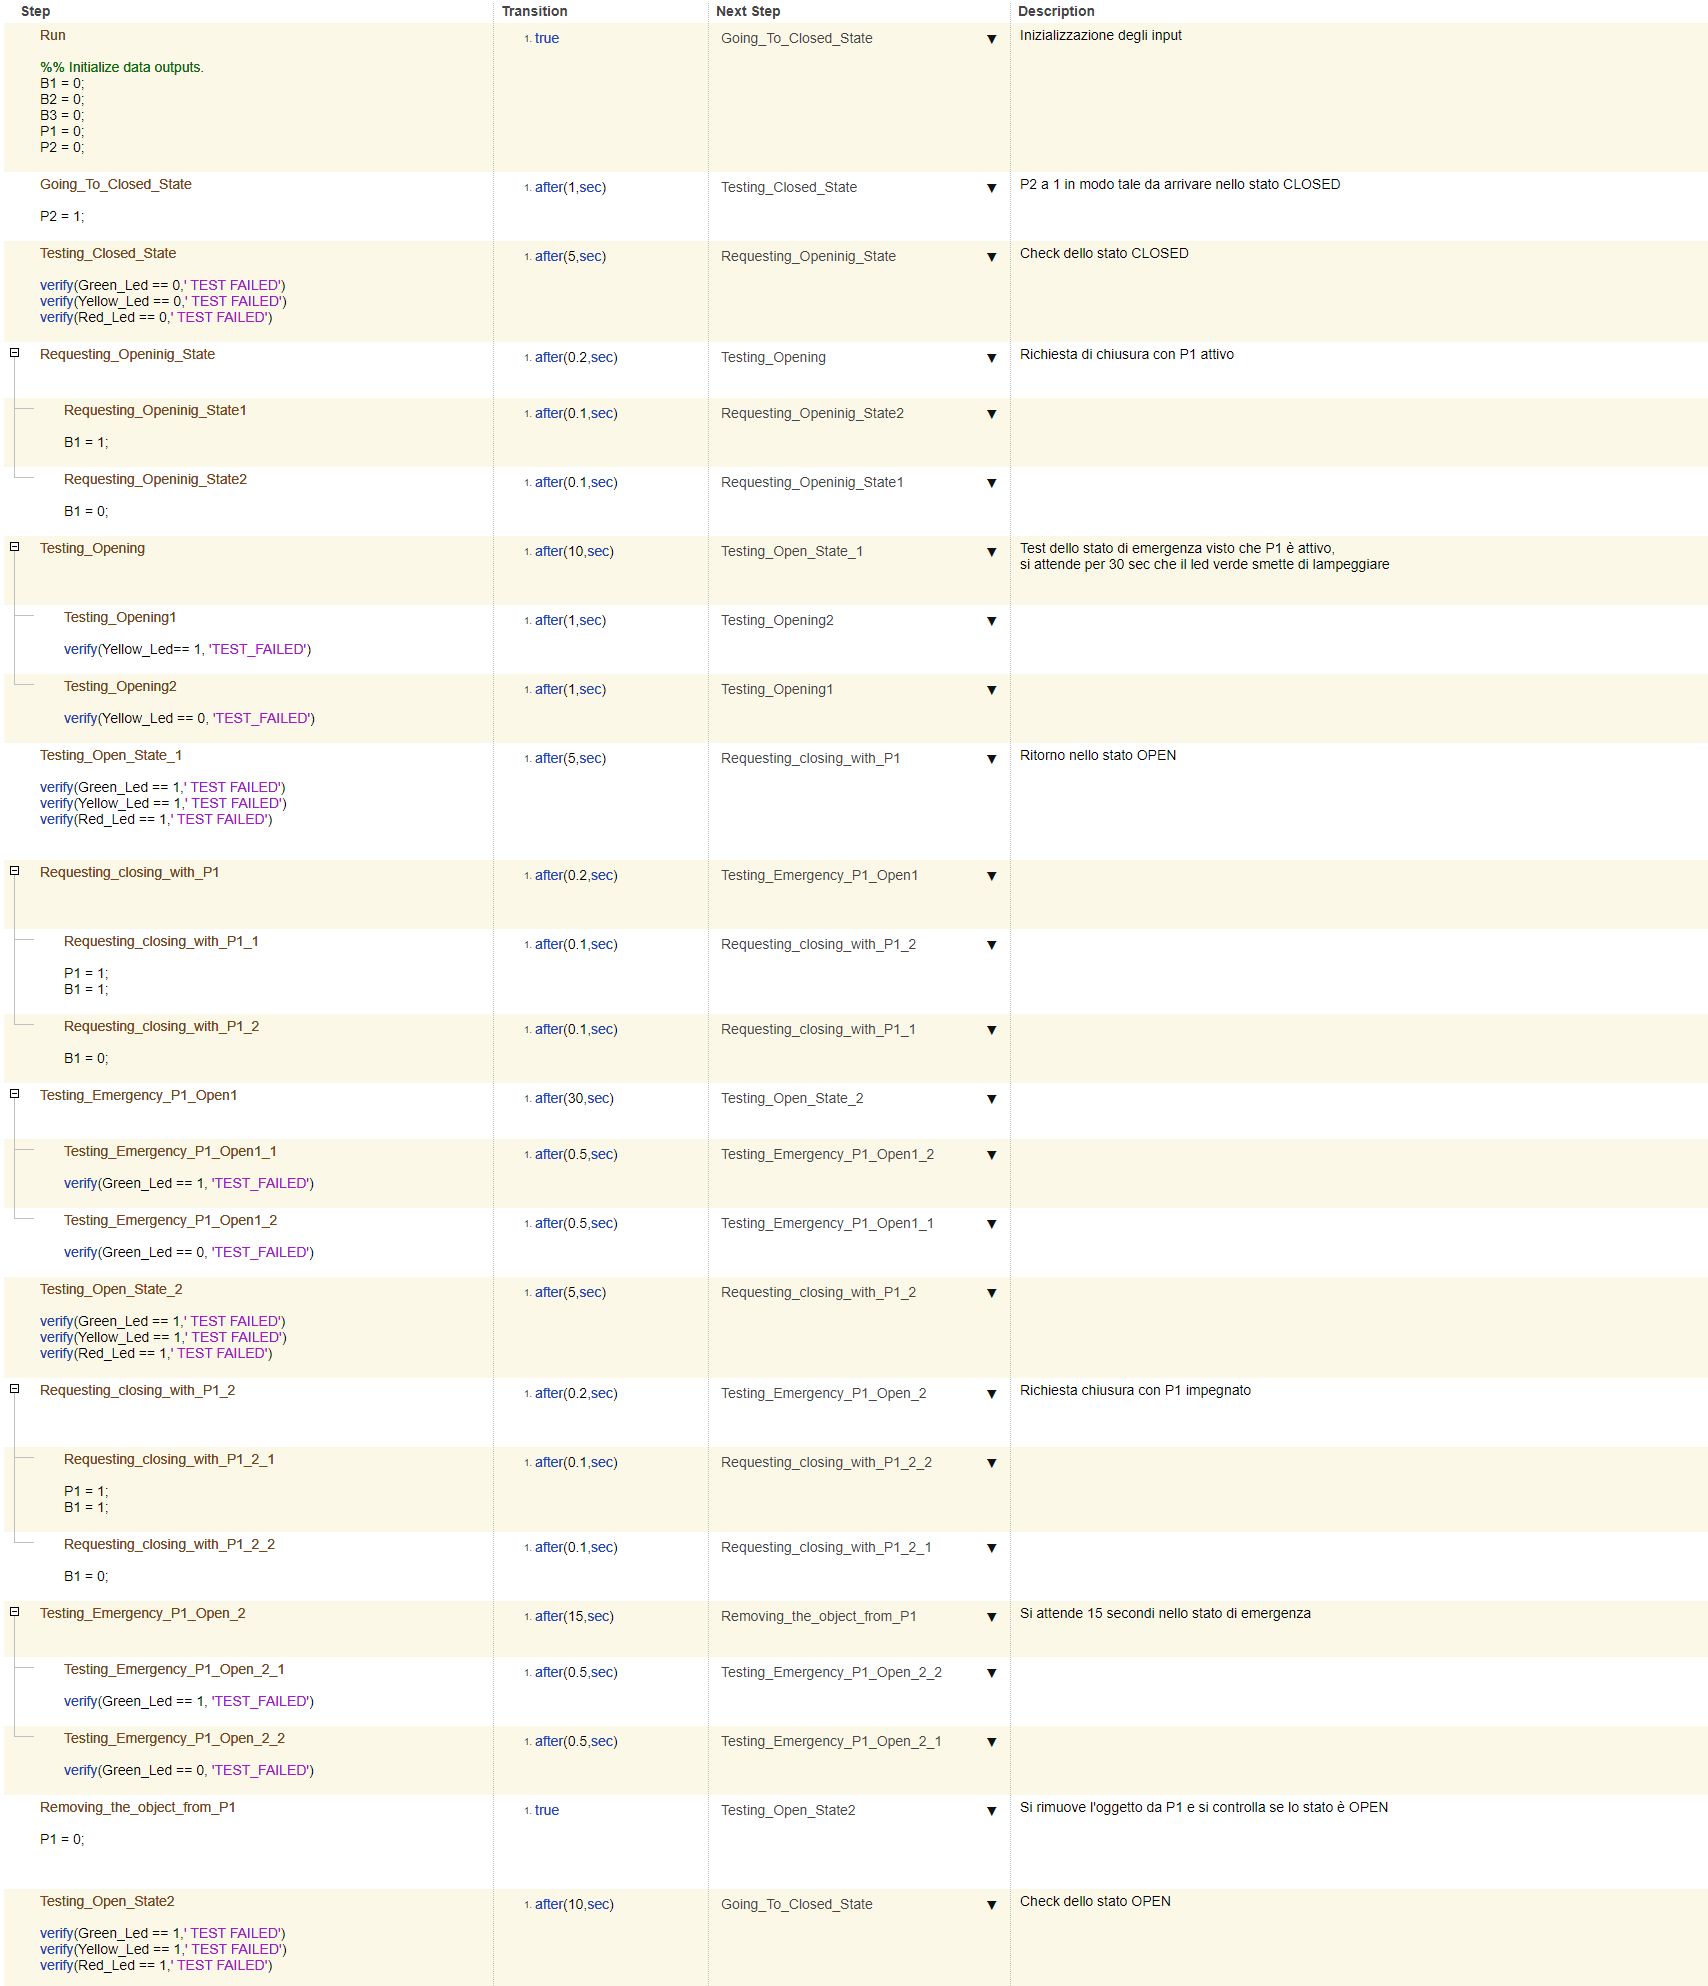
\includegraphics[width=1.3\textwidth]{Immagini_Test/Test_3_img.PNG}
    \caption{Test 3.}
    \label{fig:Test_3}
\end{figure}


\subsection{Test Case 4: Obstacle during the Closing phase}

Il test effettuato in questa sezione è molto importante nel caso in cui il sistema venisse implementato nel mondo reale, infatti controlla se il cancello automatico, che si suppone in fase di chiusura, si riapra nel caso venga rilevato un ostacolo davanti al sensore \textbf{P1}

\begin{itemize}
    \item Il sistema già parte nello stato \textbf{CLOSING} quindi non c'è bisogno di forzare alcuno stato.
    \item Viene simulata la presenza di un ostacolo attivando \textbf{P1}.
    \item Si controlla che il sistema continui ad avere il blinking del led giallo (yellow\_led) in uscita.
    \item Infine possiamo capire che il sistema è passato dalla fase di chiusura a quella di apertura intercettando lo stato finale. Se tutti i ledi sono accesi allora il test va a buon fine. 
    \item Dopo aver controllato che il sistema si trovi nello stato \textbf{OPEN} si genera l'evento che avvia la fase di chiusura, ovvero la pressione di \textbf{B1}. In questo modo il test può essere ripetuto diverse volte.
\end{itemize}

In Figura 15 sono riportate le varie fasi in Simulink Test.
\begin{figure}[H]
    
    \hspace{-2.3cm} % Sposta l'immagine di 2 cm a sinistra
    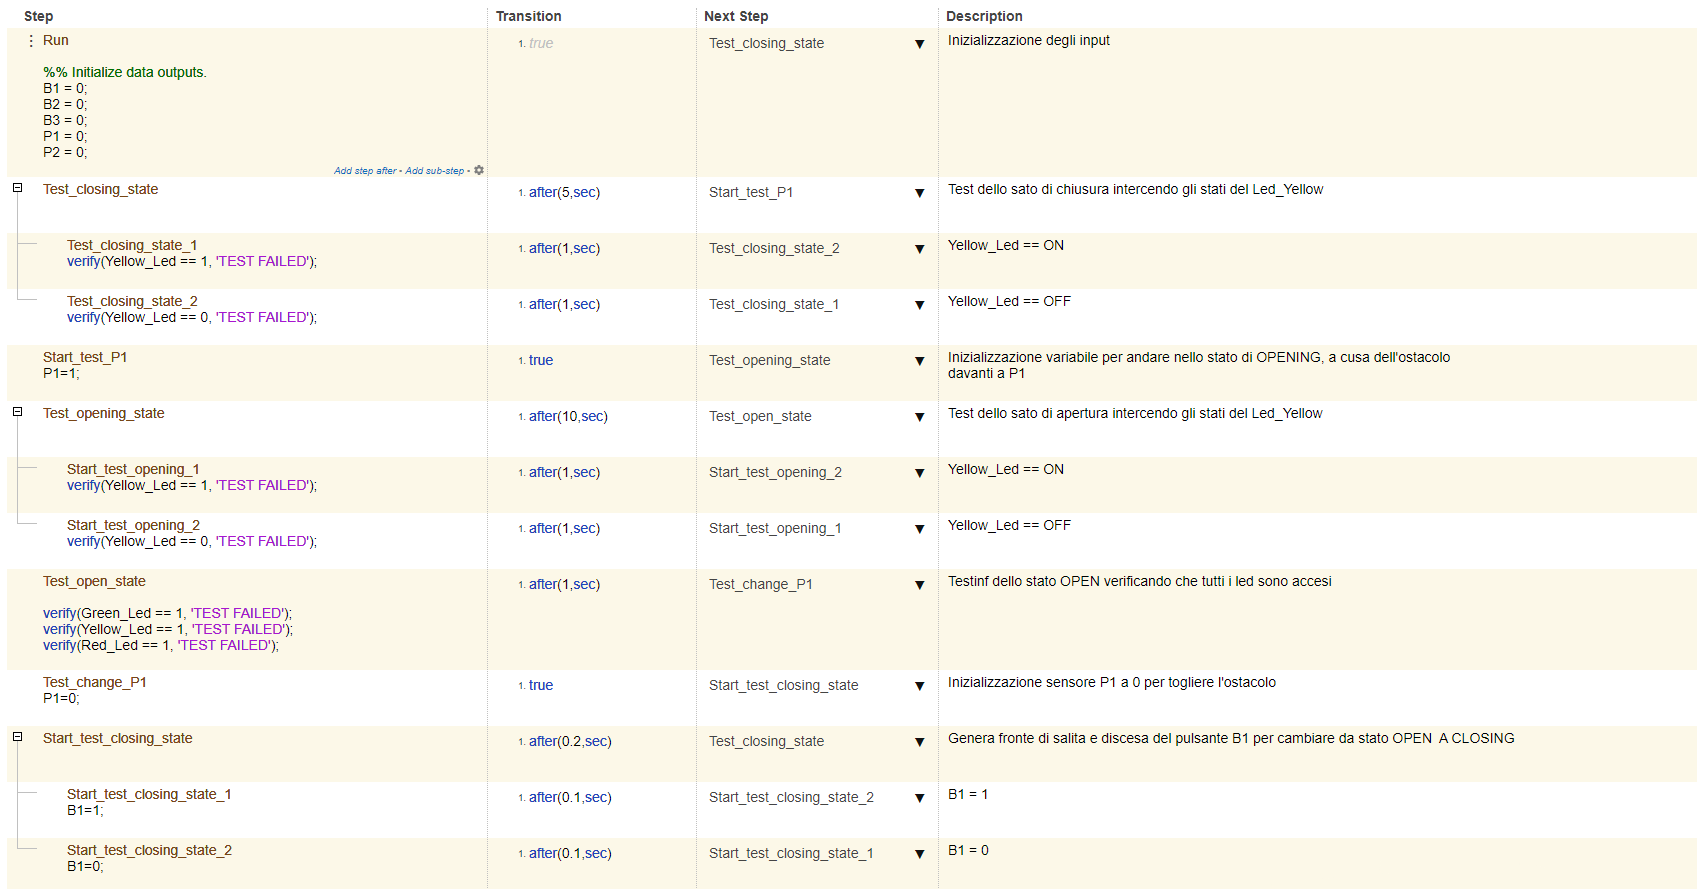
\includegraphics[width=1.3\textwidth]{Immagini_Test/Test_4_img.PNG}
    \caption{Test 4.}
    \label{fig:Test_4}
\end{figure}

\subsection{Test Case 5: Closing error (P2 is not ON)}
In questo test viene verificato che il sistema raggiunge correttamente due stati di errore nel caso in cui la chiusura del cancello automatico non avvenga nei tempi previsti definiti dall'utente.

\begin{itemize}
    \item Lo stato in cui si parte è sempre quello di \textbf{CLOSING}, in questo scenario \textbf{P2} viene attivata dopo che è passato il tempo di lavoro.
    \item Il sistema funzionante correttamente entra prima in un uno stato di errore per 10 secondi in cui tutti i led spenti.
    \item Una volta verificato lo stato precedente e passati i 10 secondi il sistema attica il led rosso (red\_led). 
    \item Successivamente si verifica che il sistema permane in questo stato fino a quando non viene attivato il sensore \textbf{P2}. Quando arriva il segnale il sistema passa nello stato \textbf{CLOSED}
\end{itemize}

Nella Figura 16 è illustrato un caso di test. È importante notare che, sebbene questo test risulti parzialmente ridondante poiché include condizioni già verificate nei controlli precedenti, esso introduce anche nuove verifiche. Si è quindi deciso di mantenere la ripetizione per aumentare ulteriormente la sicurezza del sistema.

\begin{figure}[H]
    
    \hspace{-2.3cm} % Sposta l'immagine di 2 cm a sinistra
    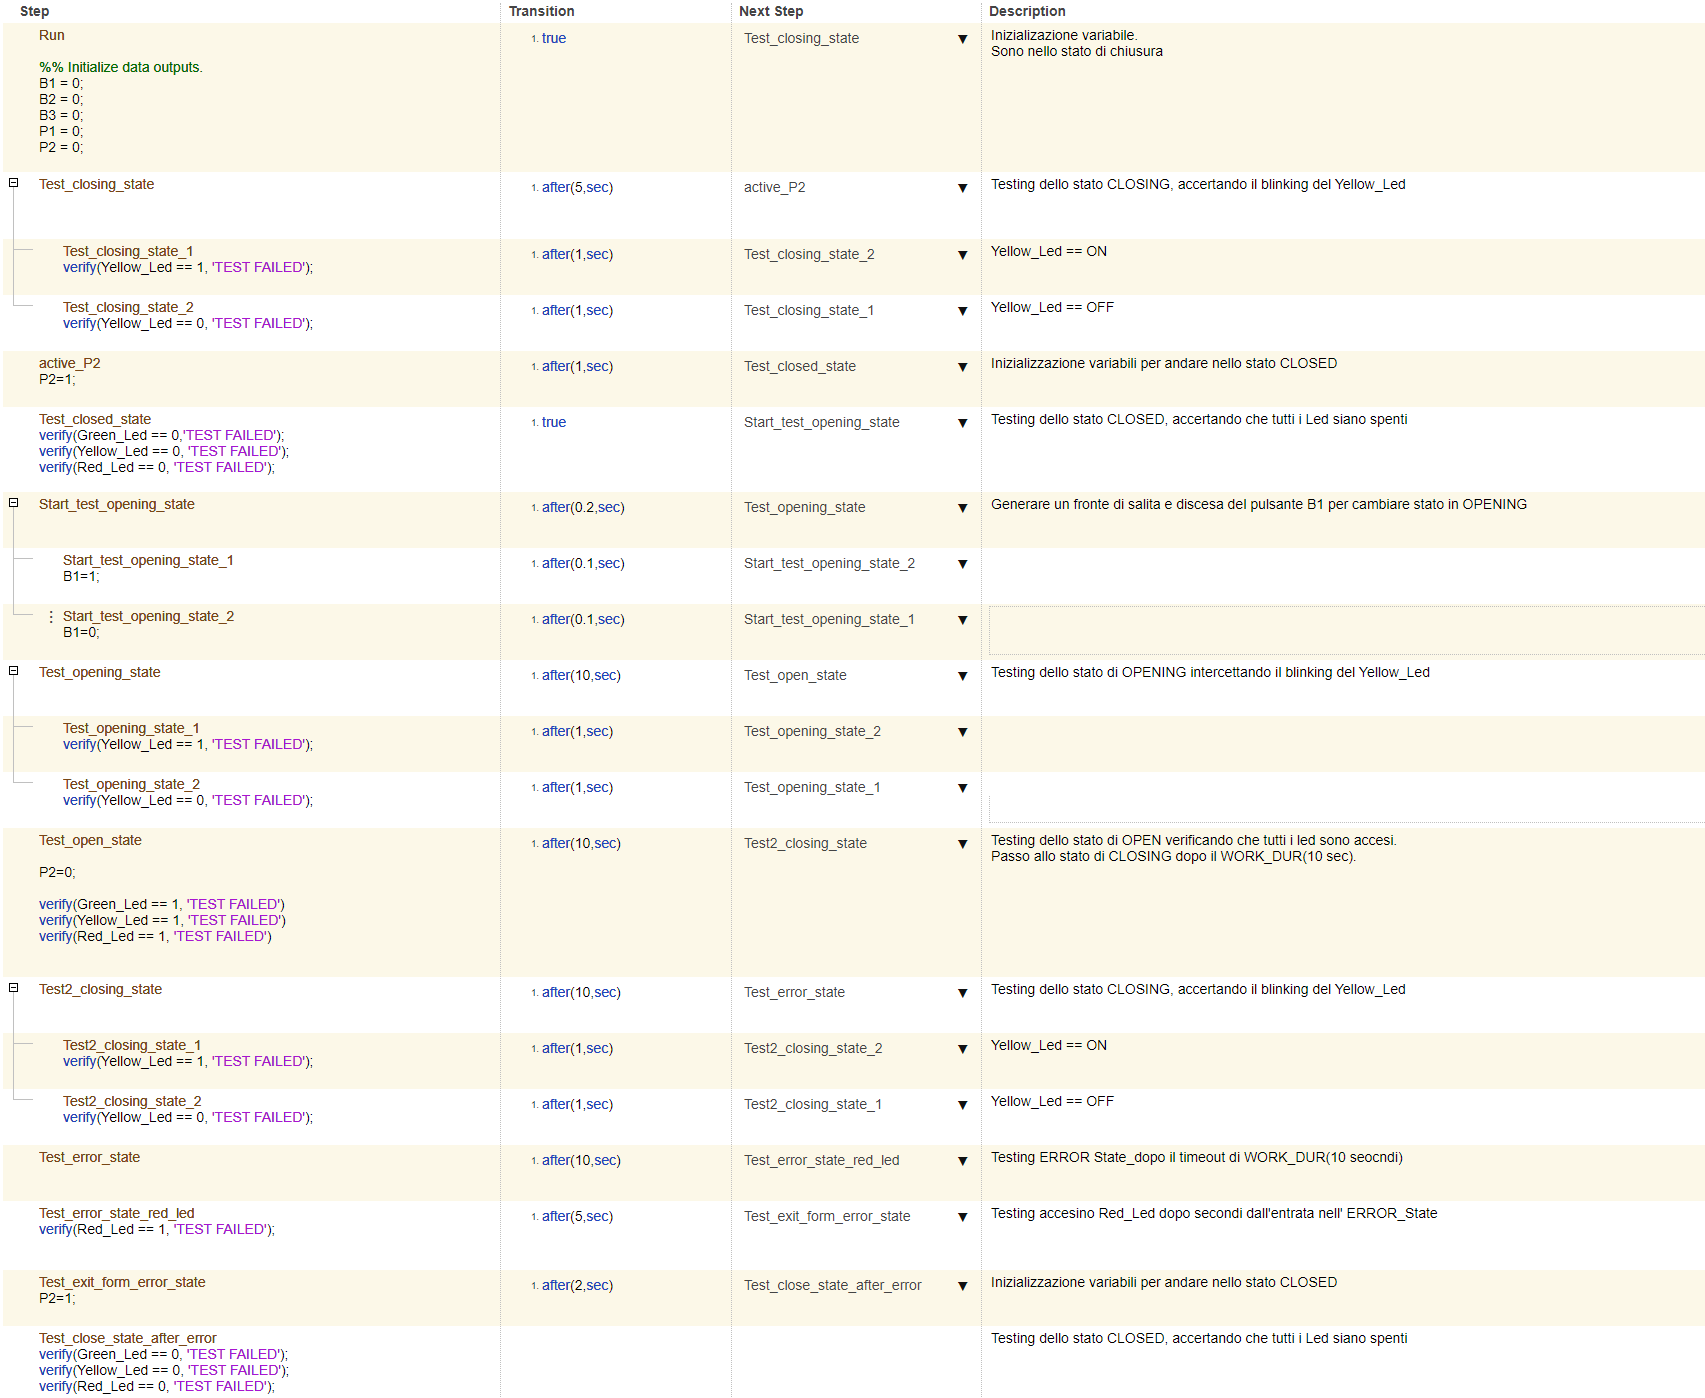
\includegraphics[width=1.3\textwidth]{Immagini_Test/Test_5_img.PNG}
    \caption{Test 5.}
    \label{fig:Test_5}
\end{figure}

\newpage
\subsection{Test Case 6: }
In questo test, viene verificato che l'impostazione del tempo di chiusura automatico e il tempo di lavoro funzionino in maniera ciclica. Una volta raggiunto il massimo tempo impostabile (120 secondi), ritorna al tempo iniziale (10 secondi).

\begin{itemize}

    \item Il cancello automatico parte da uno stato di chiusura in cui la fotocellula \textbf{P2} non rileva nulla. In questa fase viene testato il lampeggio del LED giallo (yellow LED).
    \item La fotocellula \textbf{P2} viene attivata entro il tempo di lavoro e quindi il cancello passa allo stato \textbf{CLOSED}. In questo stato si controlla che tutti i LED siano spenti.
    \item Viene richiesto l'aumento per dodici volte del tempo di chiusura automatico e del tempo di lavoro generando un fronte di salita e poi uno di discesa con il segnale dei pulsanti \textbf{B2} e \textbf{B3}.
    \item Viene richiesta l’apertura del cancello generando un fronte di salita e poi uno di discesa con il segnale del pulsante \textbf{B1}.
    \item Vengono attesi 10 secondi per verificare se la fotocellula \textbf{P2} non rileva nulla; ciò significa che il cancello è passato dallo stato di \textbf{CLOSED} allo stato di \textbf{OPEN} nel tempo desiderato.
    \item La fotocellula \textbf{P2} non viene attivata entro il tempo di lavoro e quindi il cancello passa allo stato \textbf{OPEN}. In questo stato si controlla che tutti i LED siano accesi.
    \item Quando è trascorso il tempo di chiusura automatico, impostato a 10 secondi, il sistema passa dallo stato \textbf{OPEN} allo stato di \textbf{CLOSING}. In questo modo si verifica se il tempo di chiusura è ritornato allo stato iniziale.
    \item Si verifica che il cancello passi dallo stato di \textbf{CLOSING} allo stato di \textbf{CLOSED}. Nel caso in cui non si chiuda entro 10 secondi, il sistema passa in stato di errore e dopo ulteriori 10 secondi, si verifica l'accensione del LED rosso (\textbf{Red LED}).

\end{itemize}
In Figura 17 sono riportate le varie fasi in Simulink Test.
\begin{figure}[H]
    
    \hspace{-2.3cm} % Sposta l'immagine di 2 cm a sinistra
    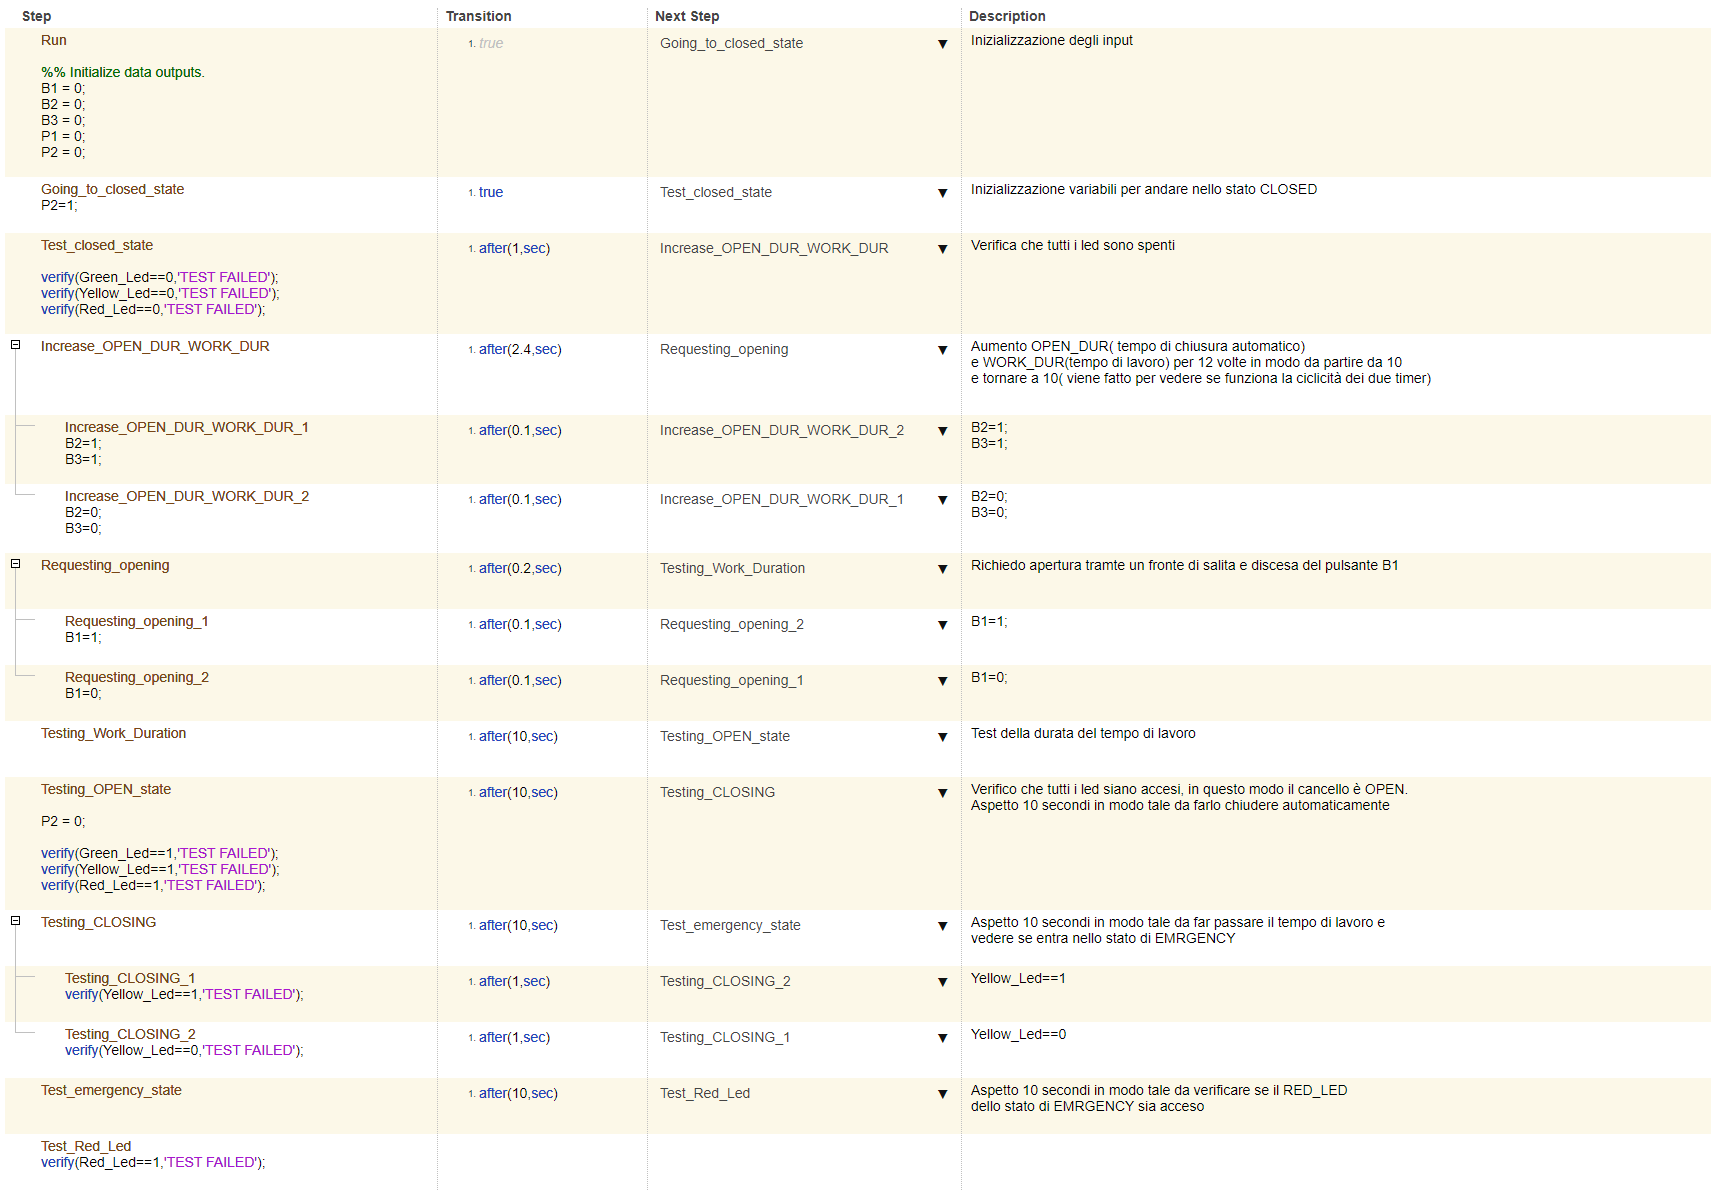
\includegraphics[width=1.3\textwidth]{Immagini_Test/Test_6_img.PNG}
    \caption{Test 6.}
    \label{fig:Test_6}
\end{figure}
\newpage
\subsection{Test Case 7: }
In questo test, viene verificato che l'impostazione del tempo di chiusura automatico e il tempo di lavoro funzioni correttamente. I tempi vengono impostati da 10 a 120 secondi per entrambi i casi tramite i relativi pulsanti.

\begin{itemize}
    \item Il cancello automatico parte da uno stato di chiusura in cui la fotocellula \textbf{P2} non rileva nulla. In questa fase viene testato il lampeggio del LED giallo (yellow LED).
    \item La fotocellula \textbf{P2} viene attivata entro il tempo di lavoro(iniziale di 10 secondi) e quindi il cancello passa allo stato \textbf{CLOSED}. In questo stato si controlla che tutti i LED siano spenti.
    \item Viene richiesto l'aumento per undici volte del tempo di chiusura automatico e del tempo di lavoro generando un fronte di salita e poi uno di discesa con il segnale dei pulsanti \textbf{B2} e \textbf{B3}. Passando cosi da 10 secondi a 120 secondi in entrambi i casi.
    \item Viene richiesta l’apertura del cancello generando un fronte di salita e poi uno di discesa con il segnale del pulsante \textbf{B1}.
    \item Vengono attesi 120 secondi per verificare se la fotocellula \textbf{P2} non rileva nulla; ciò significa che il cancello è passato dallo stato di \textbf{CLOSED} allo stato di \textbf{OPEN} nel tempo desiderato.
    \item La fotocellula \textbf{P2} non viene attivata entro il tempo di lavoro e quindi il cancello passa allo stato \textbf{OPEN}. In questo stato si controlla che tutti i LED siano accesi.
    \item Quando è trascorso il tempo di chiusura automatico, impostato a 120 secondi, il sistema passa dallo stato \textbf{OPEN} allo stato di \textbf{CLOSING}. In questo modo si verifica se il tempo di chiusura è ritornato allo stato iniziale.
    \item Si verifica che il cancello passi dallo stato di \textbf{CLOSING} allo stato di \textbf{CLOSED}. Nel caso in cui non si chiuda entro 120 secondi, il sistema passa in stato di errore e dopo ulteriori 10 secondi, si verifica l'accensione del LED rosso (\textbf{Red LED}).
\end{itemize}

In Figura 18 sono riportate le varie fasi in Simulink Test.
\begin{figure}[H]
    
    \hspace{-2.3cm} % Sposta l'immagine di 2 cm a sinistra
    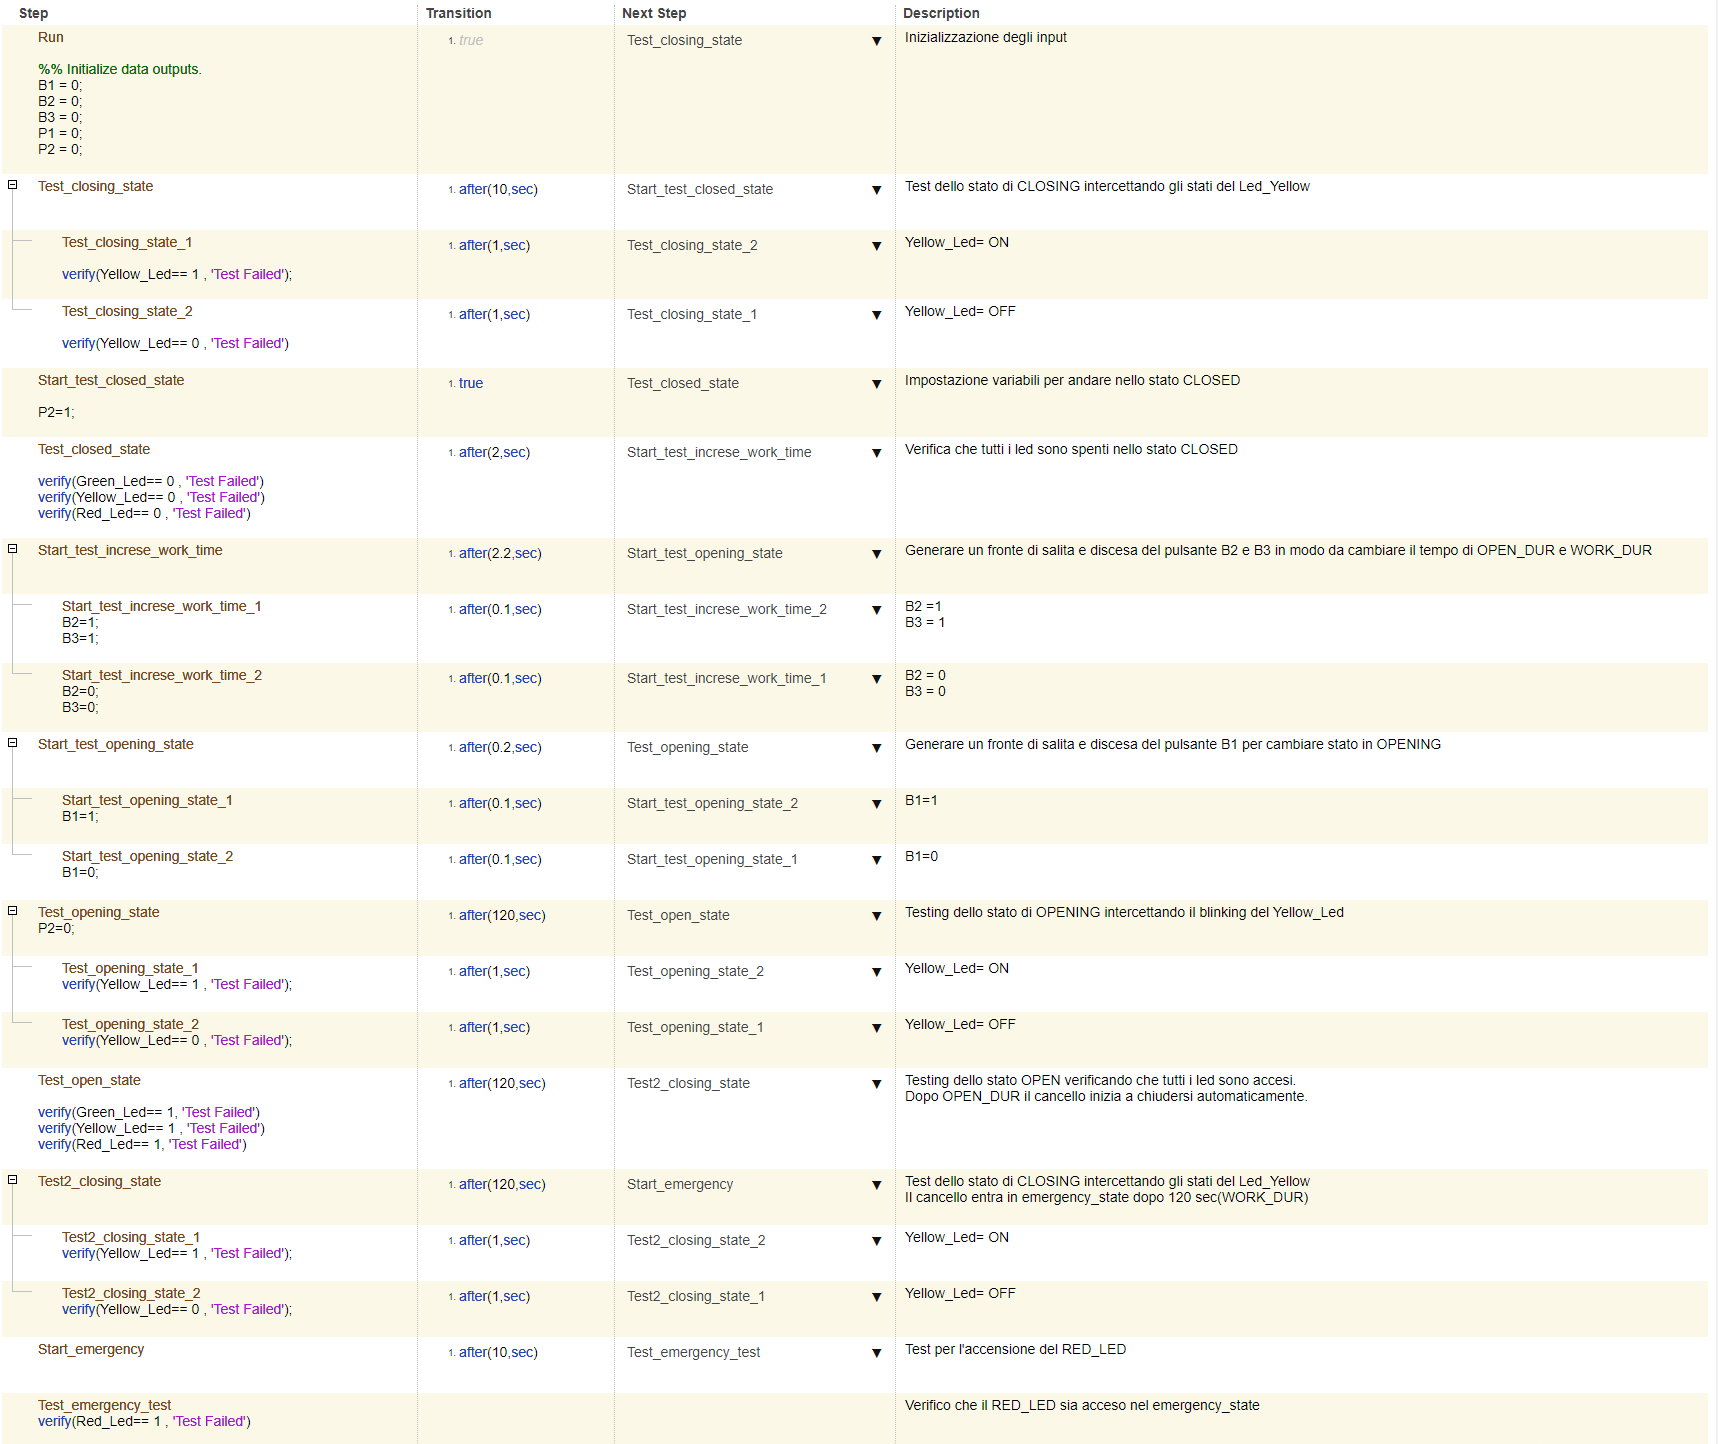
\includegraphics[width=1.3\textwidth]{Immagini_Test/Test_7_img.PNG}
    \caption{Test 7.}
    \label{fig:Test_7}
\end{figure}
\newpage
\addcontentsline{toc}{section}{Elenco delle figure}
\listoffigures
\end{document}



